\documentclass[11pt]{article}
\usepackage{amsmath, amssymb, mathtools, bm}
\usepackage{physics}
\usepackage{tikz}
\usetikzlibrary{decorations.pathmorphing,arrows.meta,calc,positioning}
\usepackage[margin=2.3cm]{geometry}
\usepackage{siunitx}
\usepackage{booktabs}
\usepackage{hyperref}
\usepackage{braket}

\newcommand{\de}{\mathrm{d}}
\newcommand{\Bext}{B_{\mathrm{ext}}}

\title{B3: Quantum, Atomic \& Molecular Physics --- Model Solutions, Trinity 2015}
\author{}
\date{}

\begin{document}
\maketitle

%==================================================================
\section*{Question 1 --- Central field, LS coupling, $5\mathrm{s}5l$ of Sr}
%==================================================================

\textbf{Problem.} Define central field approximation, configurations, terms, levels.
Derive the Land\'e interval rule.
Identify $l$ in Sr $5\mathrm{s}5l$ from three given level energies and assign $L,S,J$ to all four levels.
From six observed transition energies, identify $l'$ in $5\mathrm{s}5l'$ and assign $L,S,J$ on both ends.

\subsection*{(a) Central field approximation, configurations, terms, levels}

Replace the full electron--electron repulsion by a spherically symmetric one-body potential $U(r)$ (the spherical average of the nuclear attraction plus the mean field of the other electrons), and treat the residual
\[
H_{\rm res}=\sum_{i<j}\frac{e^{2}}{4\pi\epsilon_{0}r_{ij}}-\sum_{i}\!\bigl[U(r_{i})+Ze^{2}/(4\pi\epsilon_{0}r_{i})\bigr]
\]
as a perturbation.

In $U(r)$ each electron has good $(n,l,m_l,m_s)$ and energies $E_{nl}$, so the zeroth-order eigenstate is fully specified by populations $(nl)^{q}$ --- the \emph{configuration}.

Residual Coulomb $H_{\rm res}$ commutes with total $\bm L$ and $\bm S$ but not with individual $\bm l_i,\bm s_i$:
\[
\text{configuration}\;\longrightarrow\;\text{terms}\;{}^{2S+1}\!L,\qquad \text{splitting}\sim\SI{e4}{cm^{-1}}.
\]
Spin--orbit $H_{\rm SO}=\sum_i\xi(r_i)\bm l_i\cdot\bm s_i$ commutes only with total $\bm J=\bm L+\bm S$:
\[
\text{term}\;\longrightarrow\;\text{levels}\;{}^{2S+1}\!L_{J},\qquad J=|L-S|,\dots,L+S.
\]

\subsection*{(b) LS coupling and the Land\'e interval rule}

LS coupling: $H_{\rm res}\gg H_{\rm SO}$, so $L,S$ are good quantum numbers and $H_{\rm SO}$ acts within a fixed $^{2S+1}\!L$ term.

Project $\sum_i\xi(r_i)\bm l_i\cdot\bm s_i$ onto the term: by the projection (Wigner--Eckart) theorem,
\begin{equation}
H_{\rm SO}\big|_{LS}=A_{LS}\,\bm L\cdot\bm S.
\label{eq:HSO-LS}
\end{equation}

Use $\bm J=\bm L+\bm S$:
\[
\bm L\cdot\bm S=\tfrac12(\bm J^{2}-\bm L^{2}-\bm S^{2}).
\]

Eigenvalue in level $J$:
\[
E_{J}=\tfrac{\hbar^{2}}{2}A_{LS}\bigl[J(J+1)-L(L+1)-S(S+1)\bigr].
\]

Adjacent-level interval:
\[
E_{J}-E_{J-1}=\tfrac{\hbar^{2}}{2}A_{LS}\bigl[J(J+1)-(J-1)J\bigr].
\]

Simplify:
\begin{equation}
\boxed{\;E_{J}-E_{J-1}=\hbar^{2}A_{LS}\,J\;}
\label{eq:Lande-interval}
\end{equation}

The spacing between adjacent levels of a fine-structure multiplet is proportional to the larger $J$.

\subsection*{(c) Identifying $l$ and assigning $L,S,J$ for $5\mathrm{s}5l$}

Configuration $5\mathrm{s}5l$ has $s_{1}=s_{2}=\tfrac12$, $l_{1}=0$, $l_{2}=l$, hence $L=l$, $S=0$ or $1$:
\[
\text{four levels: }\;{}^{1}\!L_{l},\;{}^{3}\!L_{l-1},\;{}^{3}\!L_{l},\;{}^{3}\!L_{l+1}.
\]
The triplet is the only multiplet showing fine structure; the singlet is the isolated fourth level.

Triplet intervals from the data:
\[
\Delta_{1}=35022-35007=15\ \si{cm^{-1}},\qquad \Delta_{2}=35045-35022=23\ \si{cm^{-1}}.
\]
Apply \eqref{eq:Lande-interval} with $J=L,L+1$ for the two adjacent gaps:
\[
\frac{\Delta_{2}}{\Delta_{1}}=\frac{L+1}{L}.
\]
Insert numbers:
\[
\frac{23}{15}\simeq\frac{3}{2}\;\Rightarrow\;L=2.
\]

Hence $l=2$ ($5\mathrm{s}5\mathrm{d}$), and the triplet is ${}^{3}\!\mathrm{D}_{1,2,3}$.

Assignments:
\[
\boxed{\;
\begin{array}{lll}
35\,007\ \si{cm^{-1}}: &{}^{3}\mathrm{D}_{1}: & L=2,\,S=1,\,J=1,\\[2pt]
35\,022\ \si{cm^{-1}}: &{}^{3}\mathrm{D}_{2}: & L=2,\,S=1,\,J=2,\\[2pt]
35\,045\ \si{cm^{-1}}: &{}^{3}\mathrm{D}_{3}: & L=2,\,S=1,\,J=3,\\[2pt]
\text{fourth level}: &{}^{1}\mathrm{D}_{2}: & L=2,\,S=0,\,J=2.
\end{array}\;}
\]

\subsection*{(d) Identifying $l'$ in $5\mathrm{s}5l'$}

Six transitions $\Rightarrow$ a triplet--triplet multiplet with $\Delta L=\pm1,\Delta S=0,\Delta J=0,\pm1$ (no $0\!\to\!0$).

Trial $l'=1$ ($5\mathrm{s}5\mathrm{p}$, ${}^{3}\!\mathrm{P}_{0,1,2}$): selection rules give
\[
{}^{3}\!\mathrm{D}_{1}\!\to\!{}^{3}\!\mathrm{P}_{0,1,2}\;(3),\quad
{}^{3}\!\mathrm{D}_{2}\!\to\!{}^{3}\!\mathrm{P}_{1,2}\;(2),\quad
{}^{3}\!\mathrm{D}_{3}\!\to\!{}^{3}\!\mathrm{P}_{2}\;(1).
\]
Total: six. Consistent.

Cluster the data by lower level. Three transitions to the same lower level differ by the upper-${}^{3}\!\mathrm{D}$ intervals $15,23\ \si{cm^{-1}}$:
\[
20\,108,\ 20\,123,\ 20\,146:\quad\text{intervals }15,23\;\Rightarrow\;\text{common lower }{}^{3}\!\mathrm{P}_{2}.
\]
Two transitions to the same lower level differ by the upper-${}^{3}\!\mathrm{D}_{1}\!\to\!{}^{3}\!\mathrm{D}_{2}$ interval $15\ \si{cm^{-1}}$:
\[
20\,503,\ 20\,518:\quad\text{interval }15\;\Rightarrow\;\text{common lower }{}^{3}\!\mathrm{P}_{1}.
\]
Single transition:
\[
20\,689:\quad\;\text{from }{}^{3}\!\mathrm{D}_{1}\;\text{only}\;\Rightarrow\;\text{lower }{}^{3}\!\mathrm{P}_{0}.
\]

Lower-level energies:
\[
E({}^{3}\!\mathrm{P}_{2})=35\,007-20\,108=14\,899\ \si{cm^{-1}},
\]
\[
E({}^{3}\!\mathrm{P}_{1})=35\,007-20\,503=14\,504\ \si{cm^{-1}},
\]
\[
E({}^{3}\!\mathrm{P}_{0})=35\,007-20\,689=14\,318\ \si{cm^{-1}}.
\]

Land\'e check ($J=1,2$):
\[
\frac{E_{2}-E_{1}}{E_{1}-E_{0}}=\frac{14\,899-14\,504}{14\,504-14\,318}=\frac{395}{186}\simeq 2,
\]
matching $(L+1)/L=2/1$ for $L=1$, $S=1$. Confirms ${}^{3}\!\mathrm{P}$.

\[
\boxed{\;l'=1\;(5\mathrm{s}5\mathrm{p}),\qquad\text{lower }{}^{3}\!\mathrm{P}_{0,1,2}:\;L=1,\,S=1,\,J=0,1,2.\;}
\]

Per-line assignments (upper $\to$ lower):
\[
\boxed{\;
\begin{array}{ll}
20\,108\ \si{cm^{-1}}:& {}^{3}\!\mathrm{D}_{1}\;(L,S,J=2,1,1)\to{}^{3}\!\mathrm{P}_{2}\;(1,1,2),\\
20\,123\ \si{cm^{-1}}:& {}^{3}\!\mathrm{D}_{2}\;(2,1,2)\to{}^{3}\!\mathrm{P}_{2}\;(1,1,2),\\
20\,146\ \si{cm^{-1}}:& {}^{3}\!\mathrm{D}_{3}\;(2,1,3)\to{}^{3}\!\mathrm{P}_{2}\;(1,1,2),\\
20\,503\ \si{cm^{-1}}:& {}^{3}\!\mathrm{D}_{1}\;(2,1,1)\to{}^{3}\!\mathrm{P}_{1}\;(1,1,1),\\
20\,518\ \si{cm^{-1}}:& {}^{3}\!\mathrm{D}_{2}\;(2,1,2)\to{}^{3}\!\mathrm{P}_{1}\;(1,1,1),\\
20\,689\ \si{cm^{-1}}:& {}^{3}\!\mathrm{D}_{1}\;(2,1,1)\to{}^{3}\!\mathrm{P}_{0}\;(1,1,0).
\end{array}\;}
\]

%==================================================================
\section*{Question 2 --- Hyperfine structure in a magnetic field, ${}^{39}\mathrm{K}$}
%==================================================================

\textbf{Problem.}
Identify the three terms in the Hamiltonian and define weak/strong field. Show
$\Delta E_{F}=g_{F}\mu_{\rm B}\Bext M_{F}$ in the weak limit and find $g_{F}$ in terms of $g_{J}$.
Compute $g_{J}$, $F$, $g_{F}$ for ${}^{39}\!{\rm K}$ $4\mathrm{s}$.
Sketch the seven RF frequencies between hyperfine states and indicate which are visible along $\bm B$.

\subsection*{(a) Physical origin and field regimes}

\textbf{$A_{J}\,\bm I\!\cdot\!\bm J$:} hyperfine interaction. The nuclear magnetic moment $\bm\mu_{I}=g_{I}\mu_{\rm N}\bm I/\hbar$ couples to the magnetic field at the nucleus produced by the electrons; projection within a level gives $H_{\rm hf}=A_{J}\bm I\!\cdot\!\bm J$ (Fermi contact for $s$-electrons; orbital + dipolar for $l\neq 0$).

\textbf{$g_{J}\mu_{\rm B}\bm J\!\cdot\!\Bext$:} Zeeman energy of the electronic magnetic moment $\bm\mu_{J}=-g_{J}\mu_{\rm B}\bm J/\hbar$ in the external field.

\textbf{$-g_{I}\mu_{\rm N}\bm I\!\cdot\!\Bext$:} Zeeman energy of the nuclear moment in the external field; smaller than the electronic Zeeman by $\mu_{\rm N}/\mu_{\rm B}\!\sim\!10^{-3}$.

Compare the electronic Zeeman $g_{J}\mu_{\rm B}\Bext$ with the hyperfine spacing $\sim A_{J}|\bm F|$:
\[
\text{weak: }g_{J}\mu_{\rm B}\Bext\ll A_{J}\,F\;\Rightarrow\;\bm F=\bm I+\bm J\;\text{good},
\]
\[
\text{strong: }g_{J}\mu_{\rm B}\Bext\gg A_{J}\,F\;\Rightarrow\;M_{I},M_{J}\;\text{good (Paschen--Back of hfs)}.
\]

\subsection*{(b) Weak-field shift and $g_{F}$}

Couple $\bm F=\bm I+\bm J$; $|FM_{F}\rangle$ diagonalises $A_{J}\bm I\!\cdot\!\bm J$. Treat the Zeeman term as a perturbation, dropping the small nuclear Zeeman. First-order shift:
\[
\Delta E_{F}=\langle FM_{F}|g_{J}\mu_{\rm B}\bm J\!\cdot\!\Bext|FM_{F}\rangle.
\]

Project $\bm J$ onto $\bm F$ (Wigner--Eckart within a fixed $F$):
\[
\bm J\to\frac{\langle\bm J\!\cdot\!\bm F\rangle}{F(F+1)\hbar^{2}}\,\bm F.
\]

Evaluate $\bm J\!\cdot\!\bm F=\tfrac12(\bm F^{2}+\bm J^{2}-\bm I^{2})$:
\[
\langle\bm J\!\cdot\!\bm F\rangle=\tfrac{\hbar^{2}}{2}\bigl[F(F+1)+J(J+1)-I(I+1)\bigr].
\]

Take $\Bext=\Bext\hat{\bm z}$, $\langle F_{z}\rangle=\hbar M_{F}$:
\[
\Delta E_{F}=g_{J}\mu_{\rm B}\Bext M_{F}\,\frac{F(F+1)+J(J+1)-I(I+1)}{2F(F+1)}.
\]

Identify $g_{F}$:
\begin{equation}
\boxed{\;\Delta E_{F}=g_{F}\mu_{\rm B}\Bext M_{F},\qquad g_{F}=g_{J}\,\frac{F(F+1)+J(J+1)-I(I+1)}{2F(F+1)}.\;}
\label{eq:gF}
\end{equation}

\subsection*{(c) ${}^{39}\!{\rm K}$ $4\mathrm{s}$: $g_{J}$, $F$, $g_{F}$}

Ground term $4\mathrm{s}\;{}^{2}\!\mathrm{S}_{1/2}$: $L=0$, $S=\tfrac12$, $J=\tfrac12$. Land\'e formula:
\[
g_{J}=1+\frac{J(J+1)+S(S+1)-L(L+1)}{2J(J+1)}.
\]
Insert:
\[
g_{J}=1+\frac{\tfrac34+\tfrac34-0}{2\cdot\tfrac34}=1+1.
\]
\[
\boxed{\;g_{J}=2.\;}
\]

Couple $J=\tfrac12$ with $I=\tfrac32$:
\[
F=|J-I|,\dots,J+I=1,\,2.
\]

Apply \eqref{eq:gF}, $J(J+1)=\tfrac34$, $I(I+1)=\tfrac{15}{4}$:

$F=1$:
\[
g_{F}=2\cdot\frac{2+\tfrac34-\tfrac{15}{4}}{2\cdot 2}=2\cdot\frac{-1}{4}.
\]
\[
\boxed{\;g_{F=1}=-\tfrac12.\;}
\]

$F=2$:
\[
g_{F}=2\cdot\frac{6+\tfrac34-\tfrac{15}{4}}{2\cdot 6}=2\cdot\frac{3}{12}.
\]
\[
\boxed{\;g_{F=2}=+\tfrac12.\;}
\]

\subsection*{(d) Seven RF frequencies between $F=1$ and $F=2$}

Energy of a hyperfine sublevel ($\Delta F$ ignored as a constant offset between manifolds):
\[
E(F,M_{F})=E_{0}(F)+g_{F}\mu_{\rm B}\Bext M_{F}.
\]

RF transition frequency from $(F=1,M)$ to $(F=2,M')$:
\[
h\nu=h\nu_{0}+\mu_{\rm B}\Bext\bigl(g_{2}M'-g_{1}M\bigr).
\]

Substitute $g_{1}=-\tfrac12$, $g_{2}=+\tfrac12$:
\[
h\nu=h\nu_{0}+\tfrac{\mu_{\rm B}\Bext}{2}\bigl(M'+M\bigr).
\]

Magnetic-dipole selection: $\Delta F=\pm1$, $\Delta M_{F}=0,\pm1$. Tabulate $(M+M')$:
\[
\begin{array}{c|ccc}
 & M=-1 & M=0 & M=+1 \\\hline
M'=M-1\;(\sigma^{-}) & - & -1 & +1 \\
M'=M\;(\pi)         & -2 & 0 & +2 \\
M'=M+1\;(\sigma^{+})& -1 & +1 & -
\end{array}
\]

(missing entries: $M'=-2$ requires $M=-1\to M'=-2$, giving $M+M'=-3$; $M'=+2$ requires $M=+1\to M'=+2$, giving $M+M'=+3$).

Distinct values of $M+M'$:
\[
\{-3,\,-2,\,-1,\,0,\,+1,\,+2,\,+3\}\;\Rightarrow\;\boxed{\;\text{seven frequencies}.\;}
\]

\textbf{Longitudinal observation.} Along $\bm B$, only $\sigma^{\pm}$ ($\Delta M_{F}=\pm1$) radiation is emitted; $\pi$ ($\Delta M_{F}=0$) is forbidden. Visible shifts $(M+M')\in\{-3,-1,+1,+3\}$ from $\sigma$ transitions only --- four lines.

\begin{center}
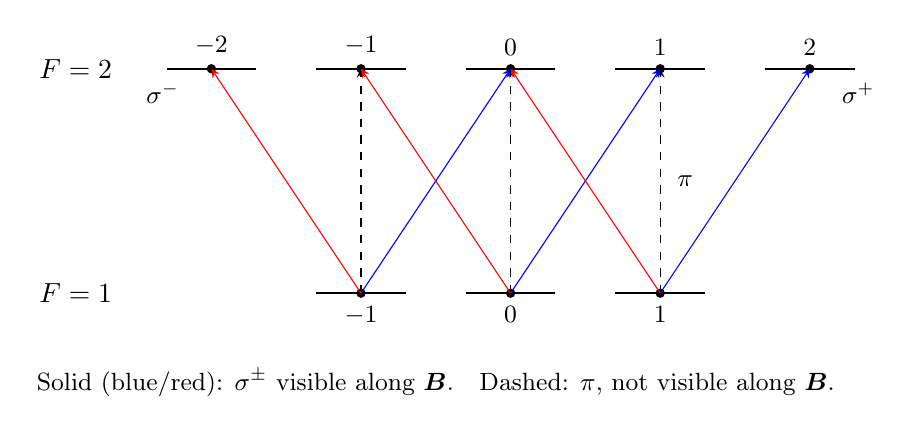
\begin{tikzpicture}[>=stealth, scale=0.95]
% F=2 level (upper)
\foreach \m/\x in {-2/-4, -1/-2, 0/0, 1/2, 2/4} {
  \draw[thick] (\x-0.6,3) -- (\x+0.6,3);
  \node[circle,fill,inner sep=1.2pt] at (\x,3) {};
  \node[above] at (\x,3.05) {\small $\m$};
}
\node[left] at (-5.2,3) {$F=2$};

% F=1 level (lower)
\foreach \m/\x in {-1/-2, 0/0, 1/2} {
  \draw[thick] (\x-0.6,0) -- (\x+0.6,0);
  \node[circle,fill,inner sep=1.2pt] at (\x,0) {};
  \node[below] at (\x,-0.05) {\small $\m$};
}
\node[left] at (-5.2,0) {$F=1$};

% pi transitions (Delta M=0): dashed (not seen along B)
\draw[dashed,->] (-2,0) -- (-2,3);
\draw[dashed,->] (0,0) -- (0,3);
\draw[dashed,->] (2,0) -- (2,3);

% sigma+ (M' = M+1): solid
\draw[->,blue] (-2,0) -- (0,3);
\draw[->,blue] (0,0) -- (2,3);
\draw[->,blue] (2,0) -- (4,3);

% sigma- (M' = M-1): solid
\draw[->,red] (-2,0) -- (-4,3);
\draw[->,red] (0,0) -- (-2,3);
\draw[->,red] (2,0) -- (0,3);

\node[above right] at (4.3,2.4) {\small $\sigma^{+}$};
\node[above left]  at (-4.3,2.4){\small $\sigma^{-}$};
\node[right] at (2.1,1.5) {\small $\pi$};
\node at (-1,-1.2) {\small Solid (blue/red): $\sigma^{\pm}$ visible along $\bm B$.\quad Dashed: $\pi$, not visible along $\bm B$.};
\end{tikzpicture}
\end{center}

%==================================================================
\section*{Question 3 --- ${}^{27}$AlH band system, P/Q/R branches}
%==================================================================

\textbf{Problem.}
Identify the terms in the rovibronic energy formula, give $\Lambda,S$ for $X^{1}\!\Sigma^{+}$ and $A^{1}\!\Pi$, derive P, Q, R-branch frequencies, locate the band head and extract $\nu_{00}$, $B'/(hc)$, equilibrium internuclear distances.

\subsection*{(a) Identifying the energy terms}

\[
E=E_{e}(R_{0})+(n+\tfrac12)h\nu_{v}+B\,K(K+1).
\]

\textbf{$E_{e}(R_{0})$:} electronic (Born--Oppenheimer) energy at the equilibrium internuclear distance $R_{0}$.

\textbf{$(n+\tfrac12)h\nu_{v}$:} vibrational energy of small-amplitude harmonic motion about $R_{0}$, $\nu_{v}=\tfrac{1}{2\pi}\sqrt{k/\mu}$, $\mu$ reduced nuclear mass.

\textbf{$B\,K(K+1)$:} rigid-rotor energy at fixed $R_{0}$, $B=\hbar^{2}/(2\mu R_{0}^{2})$, $K$ the total nuclear-rotation quantum number.

\subsection*{(b) Quantum numbers of $X^{1}\!\Sigma^{+}$ and $A^{1}\!\Pi$}

Term symbol $^{2S+1}\!\Lambda$ with $\Lambda=|L_{z}|$ (electronic orbital projection on the internuclear axis):
\[
\boxed{\;X^{1}\!\Sigma^{+}:\;S=0,\;\Lambda=0;\qquad A^{1}\!\Pi:\;S=0,\;\Lambda=\hbar.\;}
\]

\subsection*{(c) Branch frequencies}

Transition energy ($E'$ upper, $E''$ lower, $v'=v''=0$):
\[
h\nu = h\nu_{00} + B'K'(K'+1) - B''K''(K''+1).
\]

\textbf{P branch} ($\Delta K=+1$ in emission, $K''=K'+1$, hence $K'=K''-1$):

Substitute $K'=K''-1$:
\[
h\nu_{P} = h\nu_{00} + B'(K''-1)K'' - B''K''(K''+1).
\]
Expand and collect powers of $K''$:
\[
h\nu_{P} = h\nu_{00} + B'(K''^{2}-K'') - B''(K''^{2}+K'').
\]
Group:
\begin{equation}
\boxed{\;h\nu_{P}=h\nu_{00}-(B'+B'')\,K''+(B'-B'')\,K''^{2}.\;}
\label{eq:Pbranch}
\end{equation}

\textbf{Q branch} ($K'=K''$):
\[
h\nu_{Q}=h\nu_{00}+(B'-B'')\,K''(K''+1).
\]
\begin{equation}
\boxed{\;h\nu_{Q}=h\nu_{00}+(B'-B'')\,K''+(B'-B'')\,K''^{2}.\;}
\label{eq:Qbranch}
\end{equation}

\textbf{R branch} ($K'=K''+1$):
\[
h\nu_{R}=h\nu_{00}+B'(K''+1)(K''+2)-B''K''(K''+1).
\]
Expand:
\[
h\nu_{R}=h\nu_{00}+B'(K''^{2}+3K''+2)-B''(K''^{2}+K'').
\]
Group:
\begin{equation}
\boxed{\;h\nu_{R}=h\nu_{00}+2B'+(3B'-B'')\,K''+(B'-B'')\,K''^{2}.\;}
\label{eq:Rbranch}
\end{equation}

\subsection*{(d) Band head, $\nu_{00}$, $B'/(hc)$, equilibrium separations}

Treat P and R together via Fortrat parameter $m$: $m=-K''$ (P, $m\le -1$), $m=K''+1$ (R, $m\ge 1$). Both \eqref{eq:Pbranch} and \eqref{eq:Rbranch} reduce to
\[
h\nu(m)=h\nu_{00}+(B'+B'')\,m+(B'-B'')\,m^{2}.
\]

Differentiate w.r.t.\ $m$:
\[
\frac{\de(h\nu)}{\de m}=(B'+B'')+2(B'-B'')m.
\]
Set to zero:
\[
m_{\rm head}=\frac{B'+B''}{2(B''-B')}.
\]
For AlH the upper-state bond is longer, so $B'<B''$, giving $m_{\rm head}>0$: the head lies in the R branch. Translate $m_{\rm head}=K''_{\rm head}+1$:
\begin{equation}
\boxed{\;K''_{\rm head}=\frac{B'+B''}{2(B''-B')}-1.\;}
\label{eq:Khead}
\end{equation}

\textbf{Extracting $B'/(hc)$ from the Q branch.} \eqref{eq:Qbranch} written in wavenumbers ($\tilde\nu\equiv\nu/c$):
\[
\tilde\nu_{Q}(K'')-\tilde\nu_{00}=(\tilde B'-\tilde B'')\,K''(K''+1).
\]
Read from the figure: $\tilde\nu_{Q}(K''=22)\simeq 23\,200\ \si{cm^{-1}}$, and the $K''\!\to\!0$ extrapolation of the Q branch gives $\tilde\nu_{00}\simeq 23\,480\ \si{cm^{-1}}$ (this is also where Q meets the gap between R and P at low $K''$). Use $K''(K''+1)=506$:
\[
\tilde B'-\tilde B''=\frac{23\,200-23\,480}{506}.
\]
Numerator:
\[
23\,200-23\,480=-280.
\]
Divide:
\[
\tilde B'-\tilde B''=\frac{-280}{506}=-0.553\ \si{cm^{-1}}.
\]
Add $\tilde B''=6.3907\ \si{cm^{-1}}$:
\[
\boxed{\;\tilde B'\equiv B'/(hc)=5.84\ \si{cm^{-1}},\qquad\tilde\nu_{00}\simeq 23\,480\ \si{cm^{-1}}.\;}
\]

\textbf{Consistency check via R-branch head.} \eqref{eq:Khead}:
\[
K''_{\rm head}=\frac{5.84+6.39}{2(6.39-5.84)}-1=\frac{12.23}{1.10}-1.
\]
Evaluate:
\[
K''_{\rm head}\simeq 11.1-1=10.1.
\]
Head wavenumber from \eqref{eq:Rbranch} at $m_{\rm head}=11.1$:
\[
\tilde\nu_{\rm head}=\tilde\nu_{00}+(\tilde B'+\tilde B'')m_{\rm head}+(\tilde B'-\tilde B'')m_{\rm head}^{2}.
\]
Insert numbers:
\[
\tilde\nu_{\rm head}=23\,480+12.23\cdot 11.1-0.553\cdot 123.2.
\]
\[
\tilde\nu_{\rm head}=23\,480+135.8-68.1\simeq 23\,548\ \si{cm^{-1}},
\]
in agreement with the pile-up of R-branch points near $23\,545\ \si{cm^{-1}}$ in the figure.

\textbf{Equilibrium internuclear distances.} For ${}^{27}$AlH:
\[
\mu=\frac{27\cdot 1}{28}\,\si{u}=0.9643\,\si{u}=1.6014\times 10^{-27}\ \si{kg}.
\]
$B=\hbar^{2}/(2\mu R_{0}^{2})\Rightarrow B/(hc)=\hbar/(4\pi c\mu R_{0}^{2})$, hence
\[
R_{0}^{2}=\frac{\hbar}{4\pi c\mu\,(B/(hc))}.
\]

Numerator:
\[
\hbar=1.0546\times 10^{-34}\ \si{J.s}.
\]
Denominator pieces:
\[
4\pi c=4\pi\cdot 2.998\times 10^{8}=3.767\times 10^{9}\ \si{m/s}.
\]
\[
4\pi c\mu=3.767\times 10^{9}\cdot 1.6014\times 10^{-27}=6.033\times 10^{-18}\ \si{kg.m/s}.
\]
Constant prefactor:
\[
\frac{\hbar}{4\pi c\mu}=\frac{1.0546\times 10^{-34}}{6.033\times 10^{-18}}=1.748\times 10^{-17}\ \si{m^{2}.m^{-1}}.
\]

Convert $\tilde B''=6.3907\ \si{cm^{-1}}=638.07\ \si{m^{-1}}$:
\[
R_{0}''^{2}=\frac{1.748\times 10^{-17}}{638.07}=2.740\times 10^{-20}\ \si{m^{2}}.
\]
\[
R_{0}''=1.655\times 10^{-10}\ \si{m}.
\]
\[
\boxed{\;R_{0}(X^{1}\!\Sigma^{+})=1.66\ \si{\angstrom}.\;}
\]

Convert $\tilde B'=5.84\ \si{cm^{-1}}=584\ \si{m^{-1}}$:
\[
R_{0}'^{2}=\frac{1.748\times 10^{-17}}{584}=2.993\times 10^{-20}\ \si{m^{2}}.
\]
\[
R_{0}'=1.730\times 10^{-10}\ \si{m}.
\]
\[
\boxed{\;R_{0}(A^{1}\!\Pi)=1.73\ \si{\angstrom}.\;}
\]

The bond is longer in the electronically excited $A^{1}\!\Pi$ state, consistent with the smaller $B'$ inferred from the Q-branch slope and the appearance of the R-branch head.

%==================================================================
\section*{Question 4 --- X-ray transitions and K-edge filtering}
%==================================================================

\textbf{Problem.}
Interpret the Moseley-type formula and the screening constants $\sigma_n$, $\sigma_m$.
Define $K_{\alpha}$ and the K-edge; find $\sigma_{1},\sigma_{2}$ for Ca.
Derive the filter inequality and find the highest-$Z$ element whose $K_{\alpha}$ is absorbed by element $Z-1$.

\subsection*{(a) Form of the formula and the meaning of $\sigma_{n,m}$}

The hydrogenic Bohr formula for an electron in shell $n$ of nuclear charge $Z$ is $E_{n}=-hcR_{\infty}Z^{2}/n^{2}$. In a multi-electron atom an inner-shell electron sees the nuclear charge partially screened by the other electrons:
\[
Z\;\to\;Z_{\rm eff}^{(n)}=Z-\sigma_{n}.
\]
The transition energy between two such shells is the difference of effective hydrogenic levels:
\begin{equation}
E_{nm}=hcR_{\infty}\!\left[\frac{(Z-\sigma_{n})^{2}}{n^{2}}-\frac{(Z-\sigma_{m})^{2}}{m^{2}}\right].
\label{eq:Moseley}
\end{equation}

\textbf{$\sigma_{n}$:} effective screening of the nucleus by all other electrons, as seen by an electron in shell $n$ during the transition. It is approximately equal to the number of electrons whose mean radius is smaller than that of shell $n$, but is reduced by exchange/correlation and includes a partial contribution from electrons in the same shell. $\sigma_{n}$ depends on $n$ but only weakly on $Z$ (Moseley empirical rule).

\subsection*{(b) $K_{\alpha}$ and the K-edge; $\sigma$ for Ca}

\textbf{$K_{\alpha}$:} radiative transition $L\to K$ following the production of a 1s vacancy ($n=2\to n=1$, $\Delta l=\pm1$). Using \eqref{eq:Moseley} with $n=1$, $m=2$:
\[
E_{K_{\alpha}}=hcR_{\infty}\!\left[(Z-\sigma_{1})^{2}-\tfrac14(Z-\sigma_{2})^{2}\right].
\]

\textbf{K-edge:} minimum photon energy capable of ejecting a 1s electron to the continuum; the K electron's binding energy. From \eqref{eq:Moseley} with $m\to\infty$:
\[
E_{K}=hcR_{\infty}(Z-\sigma_{1})^{2}.
\]

\textbf{Calcium (Z=20).} Use $hcR_{\infty}=13.606\ \si{eV}$.

K-edge:
\[
(Z-\sigma_{1})^{2}=\frac{4039}{13.606}.
\]
Divide:
\[
(Z-\sigma_{1})^{2}=296.85.
\]
Square root:
\[
Z-\sigma_{1}=17.229.
\]
\[
\boxed{\;\sigma_{1}=20-17.23=2.77.\;}
\]

$K_{\alpha}$:
\[
\frac{E_{K_{\alpha}}}{hcR_{\infty}}=296.85-\tfrac14(20-\sigma_{2})^{2}.
\]
Insert $E_{K_{\alpha}}/(hcR_{\infty})=3692/13.606=271.41$:
\[
\tfrac14(20-\sigma_{2})^{2}=296.85-271.41=25.44.
\]
Multiply by 4:
\[
(20-\sigma_{2})^{2}=101.74.
\]
Square root:
\[
20-\sigma_{2}=10.087.
\]
\[
\boxed{\;\sigma_{2}=9.91.\;}
\]

Comment: $\sigma_{1}\simeq 2.77$ exceeds the naive value $1$ (one other K electron) because the operative screening for the $K_{\alpha}$/K-edge process includes contributions from outer electrons reorganising around the inner-shell hole. $\sigma_{2}\simeq 9.91$ is approximately the count of electrons inside the L shell plus a substantial fraction of the L electrons themselves --- reflecting that L electrons screen each other strongly in addition to the K shell.

\subsection*{(c) Filter inequality}

Efficient absorption requires the $K_{\alpha}$ photon of element $Z$ to lie above the K-edge of element $Z-1$:
\[
E_{K_{\alpha}}(Z)>E_{K\text{-edge}}(Z-1).
\]
Cancel $hcR_{\infty}$:
\[
(Z-\sigma_{1})^{2}-\tfrac14(Z-\sigma_{2})^{2}>(Z-1-\sigma_{1})^{2}.
\]
Let $a=Z-\sigma_{1}$, $b=Z-\sigma_{2}$:
\[
a^{2}-\tfrac14 b^{2}>(a-1)^{2}.
\]
Expand the RHS:
\[
a^{2}-\tfrac14 b^{2}>a^{2}-2a+1.
\]
Cancel $a^{2}$:
\[
-\tfrac14 b^{2}>-2a+1.
\]
Multiply by $-4$ (flip inequality):
\[
b^{2}<8a-4.
\]
Substitute back $a,b$:
\[
(Z-\sigma_{2})^{2}<8(Z-\sigma_{1})-4.
\]
Expand the LHS and rearrange:
\[
Z^{2}-(2\sigma_{2}+8)Z+(\sigma_{2}^{2}+8\sigma_{1}+4)<0.
\]
Solve the quadratic; take the larger root for the upper bound:
\[
Z<\tfrac{(2\sigma_{2}+8)+\sqrt{(2\sigma_{2}+8)^{2}-4(\sigma_{2}^{2}+8\sigma_{1}+4)}}{2}.
\]
Simplify by factoring 4 inside the root:
\begin{equation}
\boxed{\;Z<\sigma_{2}+4+\sqrt{(\sigma_{2}+4)^{2}-(\sigma_{2}^{2}+8\sigma_{1}+4)}.\;}
\label{eq:filter}
\end{equation}

\subsection*{(d) Highest $Z'$ and energy mismatch}

Insert $\sigma_{1}=2.77$, $\sigma_{2}=9.91$.

Outer term:
\[
\sigma_{2}+4=13.91.
\]

Inside the root:
\[
(\sigma_{2}+4)^{2}-(\sigma_{2}^{2}+8\sigma_{1}+4).
\]
Compute pieces:
\[
(\sigma_{2}+4)^{2}=13.91^{2}=193.49,
\]
\[
\sigma_{2}^{2}=9.91^{2}=98.21,\quad 8\sigma_{1}=22.16,
\]
\[
\sigma_{2}^{2}+8\sigma_{1}+4=98.21+22.16+4=124.37.
\]
Subtract:
\[
193.49-124.37=69.12.
\]
Square root:
\[
\sqrt{69.12}=8.314.
\]
Total:
\[
Z<13.91+8.31=22.22.
\]
Hence
\[
\boxed{\;Z'_{\max}=22\;(\text{Ti, filtered by Sc, }Z'-1=21).\;}
\]

\textbf{Energy mismatch} $\Delta E=E_{K_{\alpha}}(\mathrm{Ti})-E_{K\text{-edge}}(\mathrm{Sc})$.

K-edge of Sc:
\[
E_{K\text{-edge}}(21)=13.606\,(21-2.77)^{2}.
\]
Compute:
\[
(21-2.77)^{2}=18.23^{2}=332.33.
\]
\[
E_{K\text{-edge}}(21)=13.606\cdot 332.33=4521\ \si{eV}.
\]

$K_{\alpha}$ of Ti:
\[
E_{K_{\alpha}}(22)=13.606\bigl[(22-2.77)^{2}-\tfrac14(22-9.91)^{2}\bigr].
\]
Pieces:
\[
(22-2.77)^{2}=19.23^{2}=369.79,
\]
\[
(22-9.91)^{2}=12.09^{2}=146.17,\quad \tfrac14\cdot 146.17=36.54.
\]
Subtract:
\[
369.79-36.54=333.25.
\]
Multiply:
\[
E_{K_{\alpha}}(22)=13.606\cdot 333.25=4534\ \si{eV}.
\]

Difference:
\[
\boxed{\;\Delta E=E_{K_{\alpha}}(\mathrm{Ti})-E_{K\text{-edge}}(\mathrm{Sc})\simeq 4534-4521=13\ \si{eV}.\;}
\]

The $K_{\alpha}$ of Ti lies only $\sim\!13\ \si{eV}$ above the K-edge of Sc; for elements with $Z\ge 23$ (V), the $K_{\alpha}$ photon falls below the K-edge of $Z-1$ and the simple ``$Z$ filtered by $Z-1$'' rule fails.

\end{document}
